\documentclass{CFD2011}
\usepackage{CFD2011}
\usepackage{tabularx}
\usepackage{color}
%%%%%%%%%%%%%%%%%%%%%%%%%%%%%%%%%%%%%%%%%%%%%%%%%%%%%%%%%%%%%%%%%%%%%%%%%
%This template is created for complying with the author instructions for the 
%8th International Conference on CFD in Oil & Gas, Metallurgical and Process Industries
%hosted by SINTEF/NTNU, Trondheim Norway
%21-23 June 2011
%
%Sverre G. Johnsen (sverre.g.johnsen@sintef.no)
%SINTEF Materials and Chemistry


%Required files:
%   ExampleFile.tex
%   xampleFile.nls
%   CFD2011.bst
%   CFD2011.cls
%   CFD2011.sty
%   References.bib

%Example-specific files:
%   figure.eps
%   Table.tex
%%%%%%%%%%%%%%%%%%%%%%%%%%%%%%%%%%%%%%%%%%%%%%%%%%%%%%%%%%%%%%%%%%%%%%%%%


\newcommand{\Ca}{\mathrm{Ca}}

\title{Multiphase microchannel flows simulations via the lattice Boltzmann scheme}
\paperID{CFD11-52}
\author{Alexandr}{Kuzmin} %{forename}{surname}
\presenting  %the previous author is presenting the paper (name becomes underlined)
\email{shurik.kuzmin@gmail.com}%e-mail address of the previous author
\address{Chemical and Materials Engineering, University of Alberta, 9107-116 Street,  T6G 2V4
Edmonton, CANADA}%affiliation of the previous author
\author{Dmitry}{Eskin}
\email{deskin@slb.com}
\address{DBR Schlumberger Technology Center, 9450 17 Ave NW, T6N 1M9 Edmonton,CANADA}
\author{Jos}{Derksen}
%\address{NTNU Department of Physics, 7491 Trondheim, CANADA}
\email{jos@ualberta.ca}
\address{Chemical and Materials Engineering, University of Alberta, 9107-116 Street,  T6G 2V4
Edmonton, CANADA}%affiliation of the previous author


\begin{document}
\maketitle  %create the title page
\headers   %create the page headers and footers

\abstract{
In this work a free-energy binary liquid lattice Boltzmann scheme is used to simulate
Taylor/Bretherton flow in a micro-channel where elongated gas bubbles move through a liquid with
thin liquid films between the bubbles and the channel walls. The main focus of our work is a
feasibility study of the binary-liquid model lattice Botlzmann model to simulate the
Bretherton/Taylor phenomena. The numerical scheme has a diffuse
interface, and we thoroughly assess resolution requirements for correctly resolving
the liquid film and bubble motion. The simulations are two-dimensional and three-dimensional and
span a capillary number
range of $0.03$ to $0.8$ (for 2D) and range of $0.1$ to $1.0$ where the capillary number is based
on the liquid's viscosity, the
velocity of the bubble's interface, and the interfacial tension. The flow is driven by a body force,
and
periodic boundary conditions are applied in the streamwise direction. We obtain grid independent
results
as long as the liquid film thickness is at least two times the width of the diffuse interface. The
results show that the lattice Boltzmann free energy binary liquid model can be used to simulate the
Bretherton problem with a good accuracy.
}
\keywords{CFD, Multiphase Flows, Lattice Boltzmann Method, Microchannel simulations, Bretherton
Problem, Binary liquid, Free energy method}
\normalfont\normalsize

%\section{Nomenclature}
%A complete list of symbols used, with dimensions, is required.
%the nomenclature needs to be entered into the file ExampleFile.nls
\printnomenclature[0.7cm]  
\vskip .1em

\section{Introduction}
The Taylor/Bretherton \cite{bretherton} flow deals with long gas bubbles moving through liquid in
narrow channels. Depending on the geometry it was found that the deposited film thickness
is a complicated function of the capillary number $Ca$, see Eq. (\ref{capillary:number:definition}).
For example, the deposited film thickness
is proportional to $\Ca^{2/3}$ in the range of small capillary numbers for circular channels
\cite{bretherton,heil-bretherton}. 
\vskip .4em
The problem of predicting flow patterns and associated mass transfers for the Bretheron-type flows
is of significant interests for chemical industry as far as it is widely used in chemical monolith
microreactors \cite{kreutzer-pressure-drop}. While it
is possible to calculate the flow analytically for small capillary numbers \cite{bretherton}, it's
not possible to extrapolate it to the wider range of capillary numbers used in the chemical
industry. Thus, the problem of consistent numerical simulations arises.
\vskip .4em
For what follows we distinguish two- and three-dimensional cases and give a detailed description
of the literature review. 
\begin{description}
\item[2D case]
Bretherton made analytical assymptotic analysis and predicted the $\Ca^{2/3}$ dependency of the film
thickness for the circular shaped microchannels in the range of the small capillary numbers
(typically $\Ca<0.003$), where capillary number is defined as:
\begin{equation}
\label{capillary:number:definition}
\Ca=\frac{\mu_{\mathrm{liq}} U_\mathrm{bubble}}{\gamma},
\end{equation}
where $\mu_{liq}$ is the liquid viscosity, $U_{bubble}$ is the bubble velocity, and
$\gamma$ is the interfacial tension between gas and liquid. For the case of the continuous
interface models,  $U_{bubble}$ is the interface velocity.

Later on, it was realized
\cite{wong-films,wong-pressure} that the film thickness
is proportional to $\Ca^{2/3}$ only in the certain region behind the front meniscus. Overall, the
film thickness
varies over the bubble length for bubbles of finite or infinite length
\cite{heil-threedim}. Numerical
simulations \cite{giavedoni-numerical} and experimental studies
\cite{kreutzer-pressure-drop} showed a deviation from the $\Ca^{2/3}$ rule and Reynolds number 
effects on the film thickness for capillary numbers larger than $0.003$.

To consistently  predict a flow pattern for capillaries in
different ranges of the capillary number, simulations have been conducted. The simulations are
typically validated with analytical solutions in the range of the small capillary numbers
 and then extende to more practical regimes.

There are a number of numerical methods which
were used for the simulation of the Taylor/Bretherton flow.
\citet{vanbaten-circular} studied the mass transfer and film
thickness for rising bubbles in a circular capillary using the finite volume method.
\citet{kreutzer-pressure-drop} also used the finite volume method to perform
simulations of a circular capillary for a number of different
Reynolds and capillary numbers. 
\citet{heil-bretherton} and \citet{ingham-plates} studied gas finger propagation in
a two-dimensional channel for a range of Reynolds and capillary
numbers using the finite element method. \citet{giavedoni-numerical} performed cross validation of
the
finite element solution with previously published results.
The solutions were obtained for circular and planar cases. 
%The planar case results for the film
%thickness dependency on the capillary number are indicated in Fig. \ref{fig:giavedoni:planar}.
%\begin{figure}[ht]
%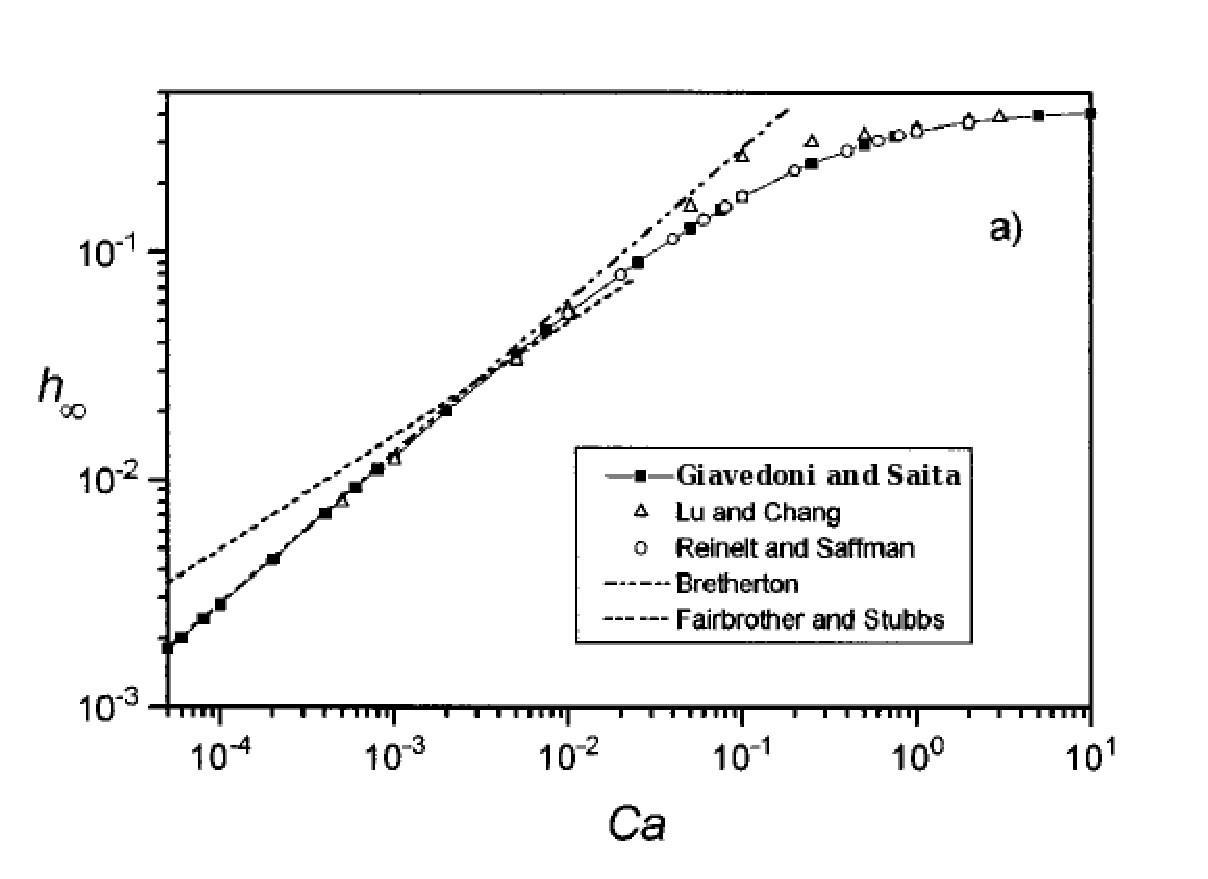
\includegraphics[width=0.5\textwidth]{Figures/giavedoni_planar.eps}
%\caption{\citet{giavedoni-numerical} gathered results across the
%literature for different capillary numbers (reprinted from \cite{giavedoni-numerical}). Results are
%scaled to the half-width of the
%channel. $h_{\infty}$ is the film thickness of gas finger at
%the infinite distance from the front meniscus. \label{fig:giavedoni:planar}}
%\end{figure} 

\item[3D case]
In comparison with the two-dimensional Bretherton flow there is a vast number of experimental
results available for the three-dimensional case. For instance, \citet{shikazono-square} obtained
experimental
results for the deposition length dependency on the
capillary number for ethanol/air and water/air mixtures and for square, circular and triangular
shaped mirochannels. \citet{cerro-bubble-train} performed a lot of experiments for a buble-train
flow in capillaries of
circular and square cross section for horizontal, upward and downward flows. The interested reader
is referred to these works for comprehensive experimental correlations.

The experimental works supported by numerical simulations reveal interesting phenomena happening in
three-dimensional geometry cases. It was found \cite{heil-threedim,wong-films} that for rectangular
or square shaped capillaries there is a transition for the
certain capillary number, where the flow changes from the non axisymmetric to axis symmetric case,
Fig. \ref{fig:sym:antisym}.
From herein, we limit ourselves to the case of microchannels with square crosssections.
Non axisymmetric case is attributed to the case where the axial radius is different from the
diagonal radius and the bubble has the non-circular shape in the channel crossection. In this case
the bubble shape mimics the shape of the square and looks like as the rounded square. The dependance
of the diagonal and axial radii on the capillary number is shown in Fig. 
\ref{fig:heil:three:dim}.
\begin{figure}[ht]
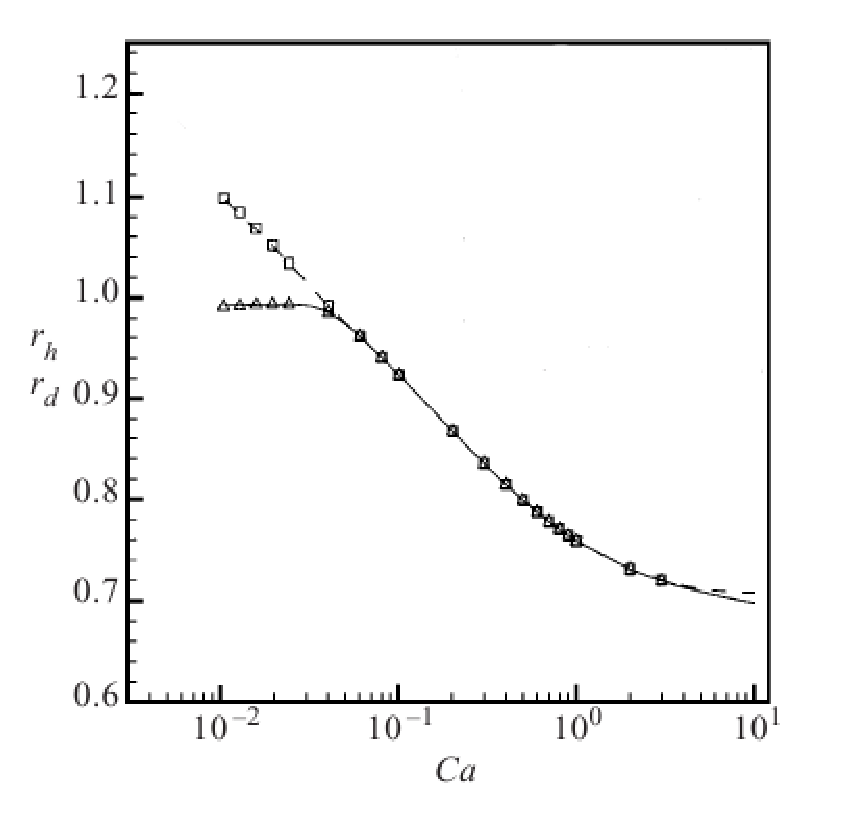
\includegraphics[width=0.5\textwidth]{Figures/capillary_width_heil.eps}
\caption{\citet{heil-threedim} results for the variation of the deposited liquid for the range of
capillary number. One can see the asymmetry between diagonal and axis diameter for the capillary
number $Ca\leq\hat{Ca}=0.04$. Courtesy of \citet{heil-threedim}. \label{fig:heil:three:dim}}
\end{figure}
The transition number between non-axisymmetric case and symmetric is indicated in a number of
works as $\widehat{Ca}=0.04$ \cite{cerro-bubble-train},
$\widehat{Ca}=0.1$
\cite{cerro-space}, $\widehat{Ca}=0.033$ \cite{heil-threedim}. If the capillary number is larger
than
the critical capillary number, i.e. $Ca>\widehat{Ca}$, then the flow becomes axisymmetric with the
radius of the droplet dependant on the capillary number. One of the example for the film
thickness dependency on the capillary number is in Fig. \ref{fig:heil:three:dim}.

\citet{heil-threedim} also indicated another interesting phenomena. They indicated the transition
capillary number where the streamlines pattern
changes from having vortex in front of the bubble and not having it for larger capilllary number,
Fig. \ref{fig:streamlines:pattern}.
For the square channel the critical number is $Ca=0.691$.   
%\begin{figure}
%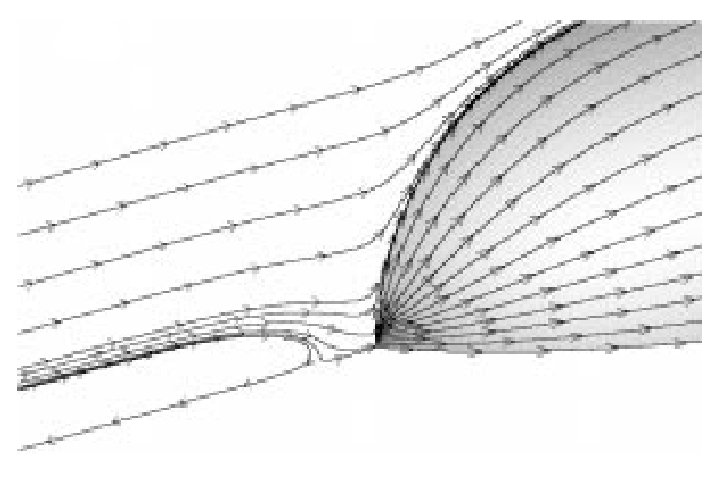
\includegraphics[width=0.5\textwidth]{Figures/ca05_clean.eps}\\
%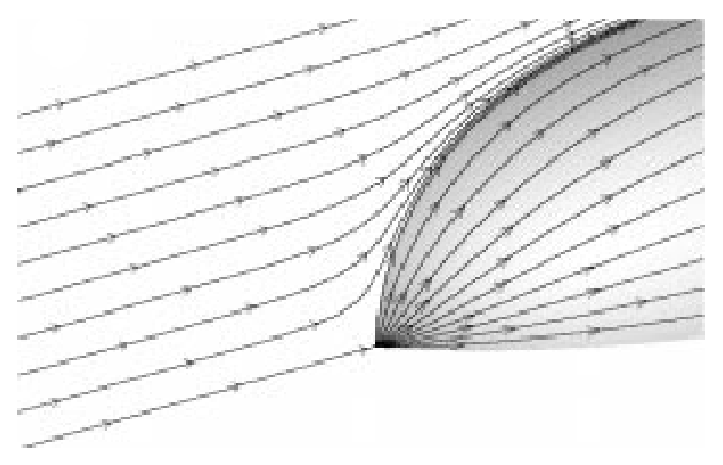
\includegraphics[width=0.5\textwidth]{Figures/ca10_clean.eps}
%\caption{Two different regimes for recirculation. Courtesy of \citet{heil-threedim}. 
%Streamlines in the moving frame of reference for a tube with $Ca = 0.5$ (top) and $Ca = 2.0$
%(bottom). 
%\label{fig:heil:recirculating}}
%\end{figure}

There are also a number of numerical works for the three-dimensional case. For instance, 
\citet{wong-films,wong-pressure} studied
three-dimensional bubbles in
polygonal capillaries and calculated bubble shapes for different
slug and bubble cross sections and menisci appearance.
\citet{heil-threedim} performed three-dimensional simulations for circular shaped,
square and rectangular shaped capillaries. Also, they investigated gravitational effects for
circular shaped capillaries. They also found the empirical correlation which allows to put
different  aspect ratio rectangular channels simulation results on one
curve. \citet{wang-non-circular} performed numerical simulations by the VOF technique for the
non-circular
shaped capillaries as square and triangular shaped capillaries. The VOF technique is the continuous
interface method based on the non-uniform grid. It is of particular interest for us to compare it
with the continuous interface method by the LBM implementation. 
They also performed
numerical simulations for the determination of the critical capillary number $\hat{Ca}$.
\end{description}
Almost all the simulations indicated above for the two-dimensional and three-dimensional cases
are performed with the help of the boundary value approach
\cite{ingham-plates,heil-bretherton,heil-threedim}. However, this method is of limited
applicability for
problems
involving complex geometries, free interface motion, or for problems involving coalescence and/or
droplet breakup. The continuous interface models are more flexible for those kind of simulations.
However, if the interface is smeared out over several grid nodes, the question of
proper film resolution in comparison with the interface resolution arises.  Therefore, the
{\emph goal} of this work is to reproduce the numerical results and phenomena presented above
with the help of the continuous interface binary liquid free energy lattice Boltzmann model. We do
a particular focus on exploring the parameter range of the binary liquid lattice
Boltzmann method for correctly resolving the flow in a range of capillary numbers. A thorough
parametric study for this approach and the ability of the
method to reconstruct consistent with other methods results has not been done to the best of the
authors' knowledge.
\vskip .5em
The lattice Boltzmann method has emerged as a successful method to simulate
a wide variety of phenomena including hydrodynamics \cite{yu}, thermal flows
\cite{karlin-minimalmodels}, microflows \cite{ansumali-small-knudsen},
ferrofluids \cite{kuzmin-aniso}, and multiphase flows
\cite{swift,Shan-chen:extended}. Thanks to its kinetic nature, LBM as a particle
method easily tackles complex geometries and allows incorporation of
physical phenomena on the microscopic level, as in the case of multiphase models. Most
multiphase lattice Boltzmann models \cite{swift, Shan-chen:extended} resolve
the interface using continuous interface methods where the interface spans over several grid nodes.
Such a representation
brings issues of the film thickness resolution versus interface
resolution -- the diffuse interface should be dealt with in such a way as to have a
negligible effect on the physics of the film.
\vskip .5em
The binary liquid free-energy LB model due to \citet{swift} we used
simulates two liquids with the assumption of uniform overall
density. While the classical Bretherton problem is stated for gas and liquid, which are of
significantly
different densities and viscosities, it was indicated \cite{bretherton} that inertia effects can be 
neglected. Moreover, the results of \citet{giavedoni-numerical} and \citet{heil-bretherton} show
negligible Reynolds number effects on the film thickness for a relatively wide range of Reynolds
numbers.
Therefore, the major governing factor for microchannel flows is not the density ratio, but the
viscosity ratio. The goal of this work is to do a feasibility assessment study of the LBM
binary-liquid model to simulate and correctly predict flow patterns for th Bretherton/Taylor
problem. The work results are in good agreement with other simulations
\cite{giavedoni-numerical,heil-bretherton,heil-threedim}.
\vskip .5em
One should also acknowledge the works of \citet{pagonabarraga-fingers} on menisci
in thin films for fingering phenomena. \citet{sehgal-microchannel} performed lattice Boltzmann
simulations of two-dimensional channel flows for a relatively large capillary numbers, and
found discrepancies with the classical Bretherton theory, which
is limited to the low capillary number regime \cite{giavedoni-numerical}.
\vskip .5em

The paper is organized as follows.  First, we briefly
explain the binary liquid lattice Boltzmann model. Then, the preliminary results for the
two-dimensional and for the three-dimensional case are presented in the results section. The paper
is
concluded with a summary of the main findings.

\section{Lattice Boltzmann binary liquid model}
The lattice Boltzmann equation (LBE) operates on a rectangular grid representing the
physical domain. It utilizes
probability distribution functions (also known as particle populations)
containing information about
macroscopic variables, such as fluid density and momentum. LBE consists of
two parts: a local collision step, and a propagation step which transports
information from one node to another in certain
directions specified by the discrete velocity set.
The LBE is typically implemented as follows:
\begin{equation}
\label{standard:implementation}
\begin{aligned}
&f_i^{*}(\bm{x},t)=\omega f_i^{eq}(\bm{x},t)-(1-\omega) f_i(\bm{x},t) +
F_i,&&\text{collision step}\\
&f_i(\bm{x}+\bm{c_i},t+1)=f_i^{*}(\bm{x},t),&&\text{propagation step}, 
\end{aligned}
\end{equation}
where $f_i$ is the probability distribution function in the direction $\bm{c_i}$, $\omega$ is the
relaxation parameter, and $F_i$ is the external force population. 

The binary fluid LB model is
based on a free-energy functional \cite{swift,landau}, and operates with two
sets of populations: one to track the pressure and the velocity fields, and another to represent the
phase field $\phi$ indicating gas or liquid.
The equilibrium populations \cite{pooley-contact} are defined as:
\begin{equation}
\label{set:equilibrium:binary}
\begin{aligned}
&f_i^{eq}&&=w_i 
\biggl(3
p_0 - k \phi \Delta \phi
+\frac{u_{\alpha}c_{i\alpha}}{c_s^2}+\frac{Q_{i\alpha\beta}u_{\alpha } u_ {
\beta}}{2 c_s^4}\biggr)\\
&&&+k w_i^{\alpha\beta} \partial_{\alpha} \phi\partial_{\beta} \phi, i=1\div Q-1\\
&f_0^{eq}&&=\rho-\sum_{i\neq0}{f_i^{eq}}\\
&g_i^{eq}&&=w_i\left(\Gamma \mu + \frac{\phi c_{i\alpha} u_{i\alpha}}{c_s^2}+\phi
\frac{Q_{i\alpha\beta}u_{\alpha}u_{\beta}}{2 c_s^4}\right), i=1\div Q-1\\
&g_0^{eq}&&=\phi-\sum_{i\neq0}{g_i^{eq}}\quad,
\end{aligned}
\end{equation}
where $\Gamma$ is the mobility parameter; the chemical potential
$\mu=-A\phi+A\phi^3-k\Delta\phi$; $k$ is the parameter related to the surface
tension; $A$ is the parameter of the free-energy model; $Q$ is the number of the directions ($9$ and
$19$ for the $D2Q9$ and $D3Q19$ models, correspondingly); the tensor
$Q_{i\alpha\beta}=c_{i\alpha} c_{i\beta} - c_s^2 \delta_{\alpha\beta}$ with
the sound speed parameter $c_s^2=1/3$. The bulk pressure
is expressed as $p_0=c_s^2 \rho +A (-0.5 \phi^2+0.75 \phi^4)$. The particular weights and velocity
sets for the $D2Q9$ and $D3Q15$ models are indicated in Appendix A. 

The set of equations (\ref{set:equilibrium:binary}) restores the macroscopic
fluid equations as:
\begin{equation}
\begin{aligned}
&\partial_t \rho+ \partial_{\alpha} \rho u_{\alpha}=0\\
&\rho\left(\partial_t+u_{\beta}\partial_{\beta}\right) u_{\alpha}=
-\partial_{\beta}P_{\alpha \beta} +
\nu\partial_{\beta}\left(\partial_{\alpha}u_{\beta}+\partial_{\beta} u_{\alpha}\right)\\
&\partial_t \phi + \partial_{\alpha} \phi u_{\alpha}=M \partial^2_{\beta\beta} \mu,
\end{aligned}
\label{binary:fluid:system}
\end{equation}
where $\nu=c_s^2 (\tau-1/2)$ is the viscosity,
$M=\Gamma(\tau_{\phi}-1/2)$ is the mobility parameter, and $\tau=\frac{1}{\omega}$ and $\tau_{\phi}$
are the relaxation parameters of density and phase fields. 

The system allows the separation of the liquid
phase with $\phi=1$ and a so-called gas phase with $\phi=-1$. The
relaxation time is taken as linearly dependent on the relaxation
times $\tau_{\mathrm{gas}}$ and $\tau_{\mathrm{liq}}$:
$\tau=\tau_{\mathrm{gas}}+\frac{\phi+1}{2}(\tau_{\mathrm{liq}}-\tau_{\mathrm{gas}})$. This allows
to change viscosity from the gas viscosity
$\nu_{\mathrm{gas}}=\frac{1}{3}\Bigl(\tau_{\mathrm{gas}}-\frac{1}{2}\Bigr)$ to the liquid viscosity
$\nu_{\mathrm{liq}}=\frac{1}{3}\Bigl(\tau_{\mathrm{liq}}-\frac{1}{2}\Bigr)$ while phase changes
accordingly.The surface tension in the framework of the binary liquid model is $\sqrt{\frac{8 k
A}{9}}$.

\section{Numerical benchmark}
To be able to properly simulate and compare simulation results with data
published in the literature, one needs to design a numerical benchmark addressing
all the challenges for the lattice Boltzmann method. That includes the diffuse nature of the
interface which needs to have a negligible effect on the results. Also, as far as the density is
uniform, the binary liquid model can address only different viscosities of gas and liquid.
Another challenge is boundary conditions because one needs to couple inlet and outlet
boundary conditions \cite{heil-threedim} for the film thickness to establish.  The geometry of
the problem is also of concern. Most literature numerical simulations are done for a channel with
circular cross section,
which is quite difficult to address in terms of lattice Boltzmann framework. We thoroughly discuss
all the
challenges associated with the lattice Boltzmann microchannel simulations in our recent work
\cite{kuzmin-binary2d}. 

Given all the concerns and challenges, the suggested lattice Boltzmann framework
is a two-dimensional flow between plates and three-dimensional square
shaped microchannels, both driven by a body force. We limit ourselves to the study
of body force driven flows, because of their simplicity and better numerical stability. This
implies that we can use the periodic boundary conditions in the streamwise direction. As soon as the
periodic boundary
conditions are applied, not a single bubble but a bubble train is simulated. In this case one
needs
to ensure that the distance between bubbles is large enough to exclude mutual bubble influence. 
Therefore, we chose the bubble length to be $5$ channel heights. This number is shown
to be sufficient to give results consistent with the theory. The
channel length is taken to be $3$ bubble lengths (or $15$ channel heights)
to minimize influence of one bubble on another,
because of the periodicity of boundary conditions. The geometry
dimensions are represented in Fig. \ref{fig:benchmark:sketch}.
\begin{figure}[ht]
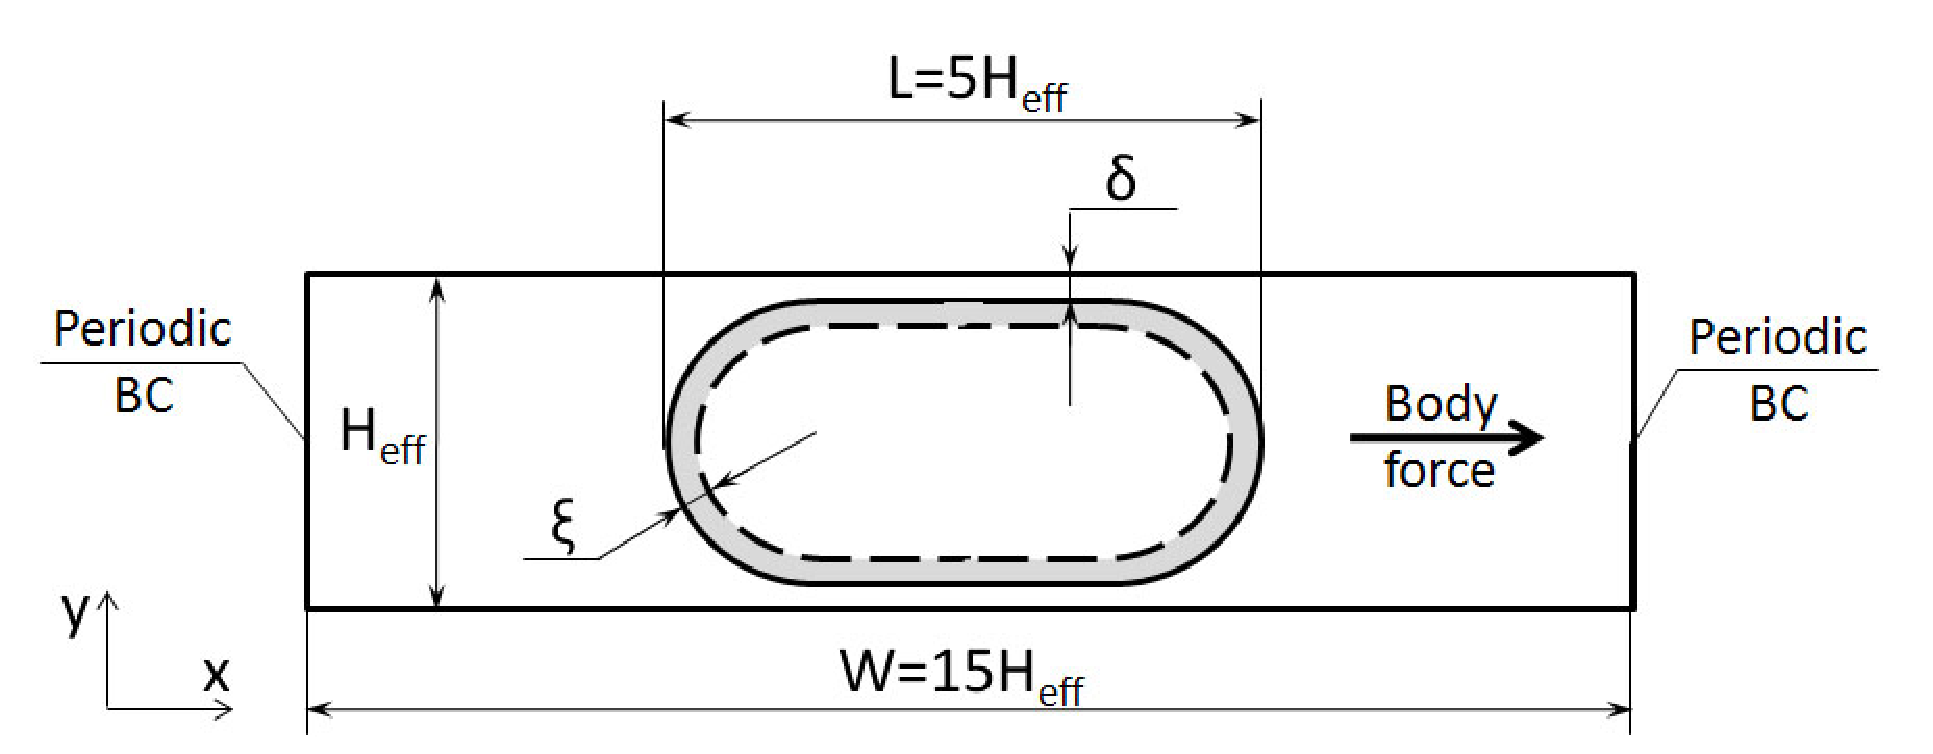
\includegraphics[width=0.5\textwidth]{Figures/benchmark.eps}
\caption{The two-dimensional benchmark sketch. $\delta$ corresponds to film thickness. $5\xi$
corresponds to the interface thickness. We take the microchannel length to be $15$ times larger than
its height. The threedimensional benchmark has the same geometry extending one dimension to have a
square shaped crosssection.
\label{fig:benchmark:sketch}}
\end{figure}

\section{Results}
\subsection{2D results}
Two-dimensional binary-liquid simulations are presented in our recent work
\cite{kuzmin-binary2d}. Here we outline two most important results. The first one addresses the
question of how the interface should be resolved to obtain grid independent result. Though the
simulations are performed for the lattice Boltzmann model, the results can be applied for any
uniform grid continuous interface method. The second part of results are comparisons with the
literature results for the film thickness dependency on the capillary number.
 
\subsubsection{Grid refinement}
To properly estimate the interface resolution one needs to study the convergence as a function of
the grid resolution. To do that the grid resolution is varied while all remaining parameters,
including the bubble velocity and the capillary number, are fixed.  Our goal is to determine the 
ratio of the interface thickness to the 
film thickness at which results are no longer dependent on the grid resolution.


We performed a number of simulations for grids indicated in
Table \ref{table:parameters:grid:refinement}. Other parameters are defined as $k=0.04$, $A=0.04$ and
$\Gamma=1.0$. Note that in the case of the half-way bounce-back walls \cite{yu} which are used in
the
simulations one needs to calculate the film thickness as:
\begin{equation}
\delta=(\phi_0-0.5)/(N_y-2)=(\phi_0-0.5)/H_{\mathrm{eff}},
\end{equation}
where $\phi_0$ is the grid coordinate where phase field is $0$, $H_{\mathrm{eff}}=N_y-2$
is the effective channel height.
If the grid size in the $y$ direction is $N_y$, then one has $N_y-1$ regions between the grid nodes
which represent
the physical domain, top and bottom nodes are bounce-back nodes. Then the effective wall location is
in the middle between bounce-back and fluid
nodes. Overall there are $N_y-2$ nodes representing the fluid. Note that it is a big
simplification to impose the boundary in the middle between the bounce-back
node and the fluid node. The location of the wall for bounce-back nodes is
viscosity dependent \cite{ginzburg-multireflection}.  However, the effective location of the
wall for the
multiphase models to the best authors' knowledge is not yet derived.
The bubble is initialized as a rectangular box with coordinates
$y=7\times\frac{H_\mathrm{eff}}{100}\dots N_y-7\times\frac{H_\mathrm{eff}}{100}-1$,
$x=\frac{N_x}{3}\dots \frac{2 N_x}{3}$ and phase
$\phi_{\mathrm{bubble}}=-1$. All other nodes are initialized with the phase field
$\phi=1$. The initialization procedure is done to keep the self-similarity. The initial width and
body force were chosen to aim for the capillary number $\Ca=0.05$ \cite{kuzmin-binary2d}.
After choosing the reference parameters, the grid refinement procedure
needs to keep the macroscopic parameters constant.  It is easy to check
that it yields the following quantity to
be independent of grid size
$H_{\mathrm{eff}}^2\frac{\mathrm{d}P}{\mathrm{d}x}=(N_y-2)^2\frac{\mathrm{d}P}{\mathrm{d}
x } = \mathrm{const}$. For the grid $H_{\mathrm{eff}}=100$ we chose the body force as
$\frac{\mathrm{d}P}{\mathrm{d}x}=1.508 \times 10^{-6}$ lattice units.
The
simulation results in terms of the film thickness $\delta$, interface bubble
velocity $U_{bubble}$ and associated capillary numbers are summarized in Table
\ref{table:parameters:grid:refinement}. 
The unified scaled profiles are shown in Fig. \ref{fig:grid:profiles}. One can
see that results converge for $H_{\mathrm{eff}}\geq 175$. To calculate how well the interface is
resolved, the ratio of the interface thickness to the film thickness is calculated. The
interface itself occupies approximately $5 \xi$, where
$\xi=\sqrt{k/A}=1$. The ratio of the interface thickness to the film thickness
$5\xi/H_{\mathrm{film}}$ is shown in Table \ref{table:parameters:grid:refinement}.

Based on these results one can conclude
that
 the interface needs to be resolved as $40-50$ percent of the
expected film thickness for simulations to be grid independent. We further examine the
velocities in the center of the bubble to calculate the capillary number. One can see from Table
\ref{table:parameters:grid:refinement} that the bubble velocities are consistent and the
calculated capillary number corresponding to these velocities is $0.07$.
\begin{figure}[ht]
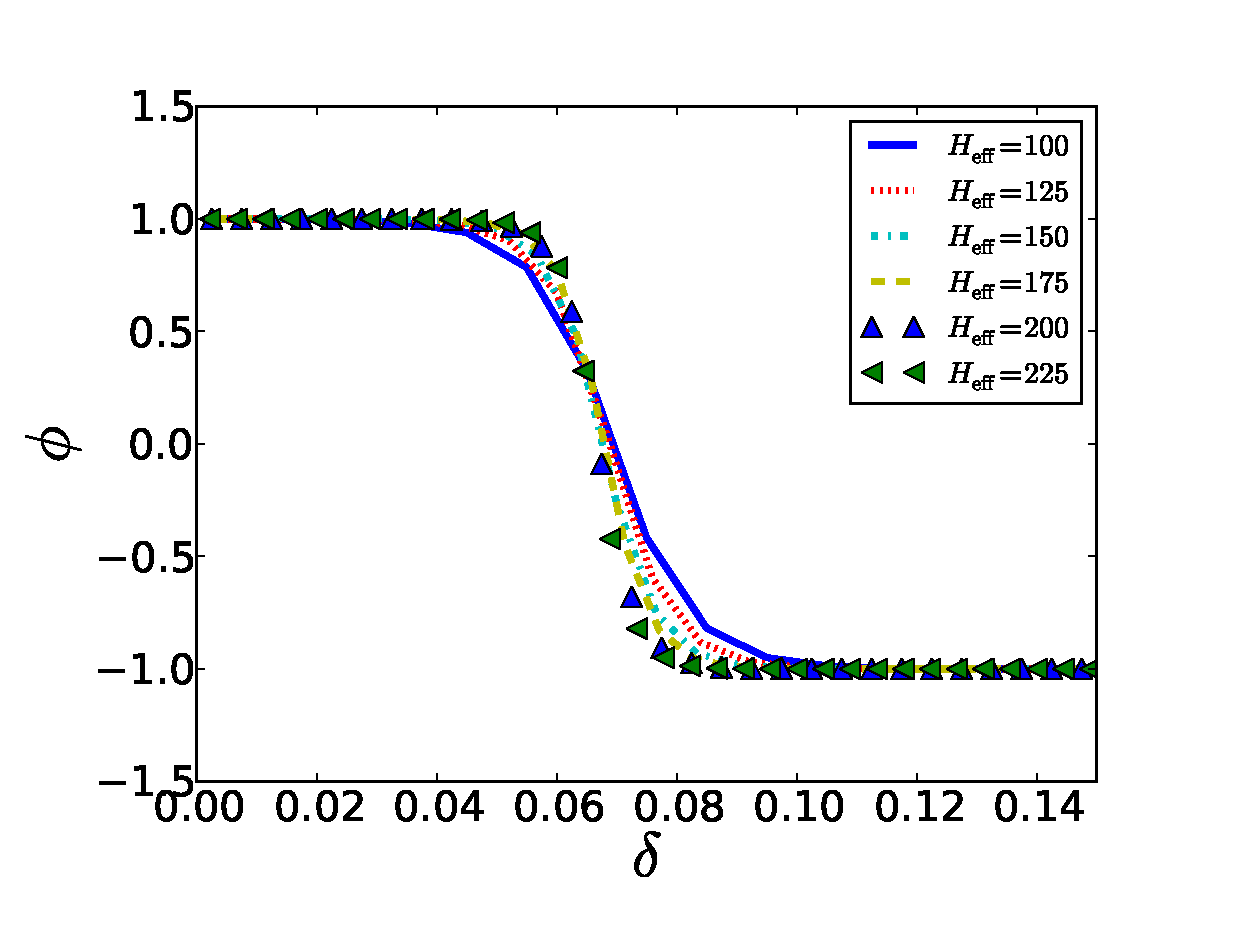
\includegraphics[width=0.5\textwidth]{Figures/norm_grid_profs.eps}
\caption{Grid-refined profiles for the effective
channel widths
$H_{\mathrm{eff}}=100,125,150,175,200,225$. $\delta$ is scaled on $H_{\mathrm{eff}}$ and $\delta=0$
corresponds to the wall location. The profiles were taken at $x=14$ (nondimensional coordinates).
Capillary number we aim for is $\Ca=0.05$. The capillary number obtained from simulations
$\Ca=0.07$. 
\label{fig:grid:profiles}}
\end{figure}
\begin{table}
\begin{tabularx}{0.5\textwidth}{|X|X|X|X|X|X|}
\hline
$N_x$&$N_y$&$\delta$&$U_\mathrm{bubble}$&$\frac{5\xi}{H_{\mathrm{film}}}$&$N_\mathrm{iter}$\\
\hline
$1500$&$102$&$0.0694$&$0.0041$&$0.824$&$200000$\\
\hline
$1875$&$127$&$0.0688$&$0.0041$&$0.646$&$250000$\\
\hline
$2250$&$152$&$0.0676$&$0.0040$&$0.539$&$300000$\\
\hline
$2625$&$177$&$0.0679$&$0.0040$&$0.453$&$350000$\\
\hline
$3000$&$202$&$0.0668$&$0.0041$&$0.400$&$400000$\\
\hline
$3375$&$227$&$0.0663$&$0.0039$&$0.355$&$450000$\\
\hline
\end{tabularx}
\caption{The parameters and results for grid resolution. The simulated domain is
of size $N_x \times N_y$. $U_\mathrm{bubble}$ is the interface velocity of the bubble center
measured at the front meniscus.  $5\xi$ is the interface thickness. $H_{\mathrm{film}}=\delta
(N_y-2)$ is the size of the film in
lattice Boltzmann units.
\label{table:parameters:grid:refinement}}
\end{table}

\subsubsection{Capillary number region}
The purpose of this section is to validate the correlations of
\citet{giavedoni-numerical} and
\citet{heil-bretherton} for a film thickness dependancy on the range of capillary
numbers. Because of limited computational resources, we skip the
small capillary numbers and make calculations for the range of capillary numbers $0.03-0.8$, which
is a computationally reasonable task.  To be consistent with the grid independant results, we choose
the grid to be
$202 \times 3001$. Then $5$ lattice Boltzmann units do not occupy more than $60$
percent of the effective film thickness. Because the simulation gets unstable with
smaller grids and larger gradients, all the capillary number simulations were
performed on the same grid. To properly initialize the body force, the
proportionality law was utilized. The forcing
$6 \cdot 10^{-6}/16$ was chosen to obtain the predicted capillary
number $0.05$. The forcing for other grids can be obtained using
simple proportionality relationships:
\begin{equation}
\begin{aligned}
&\Ca_{\mathrm{lit}} \propto U_{\mathrm{bubble}}\\
&U_{\mathrm{bubble}} \propto \frac{\mathrm{d}P}{\mathrm{d}x} N_y^2\\
&\Ca_{\mathrm{lit}} \propto \frac{\mathrm{d}P}{\mathrm{d} x} N_y^2 \text{ or }\\
&\frac{\mathrm{d}P}{\mathrm{d} x} \propto \frac{\Ca_{\mathrm{lit}}}{N_y^2},
\end{aligned}
\end{equation}
where the subscript ,,lit'' stands for the predicted capillary number
\cite{giavedoni-numerical,heil-bretherton}. The grid number $N_y$ is not
involved because all simulations are conducted on the same grid.
The pressure gradient can be obtained through the capillary number
ratio:
\begin{equation}
\frac{\mathrm{d}P}{\mathrm{d} x}=6 \cdot 10^{-6}/16 \frac{\Ca_{\mathrm{lit}}}{0.05}
\end{equation}
The film thickness is initialized through the ratio of capillary numbers as well:
\begin{equation*}
w=12 \frac{\Ca_{\mathrm{lit}}}{0.05}
\end{equation*}
The results obtained after $2\cdot10^5$ steps are presented in Table
\ref{table:parameters:capillary:number}. One can see that the calculated
capillary numbers are overpredicted but the obtained thicknesses are overpredicted
as well due to the body force setting caused by the Poiseuille flow assumption. If one
needs to obtain the desired capillary number, the shooting method for the forcing is
necessary, starting with the Poiseuille pressure gradient force as the initial condition. We
extracted
the data of 
\citet{giavedoni-numerical} and \citet{heil-bretherton} with the help of software ``Engauge
Digitizer'' and compared them with our results (see 
Fig. \ref{fig:capillary:comparison}).
\begin{figure}
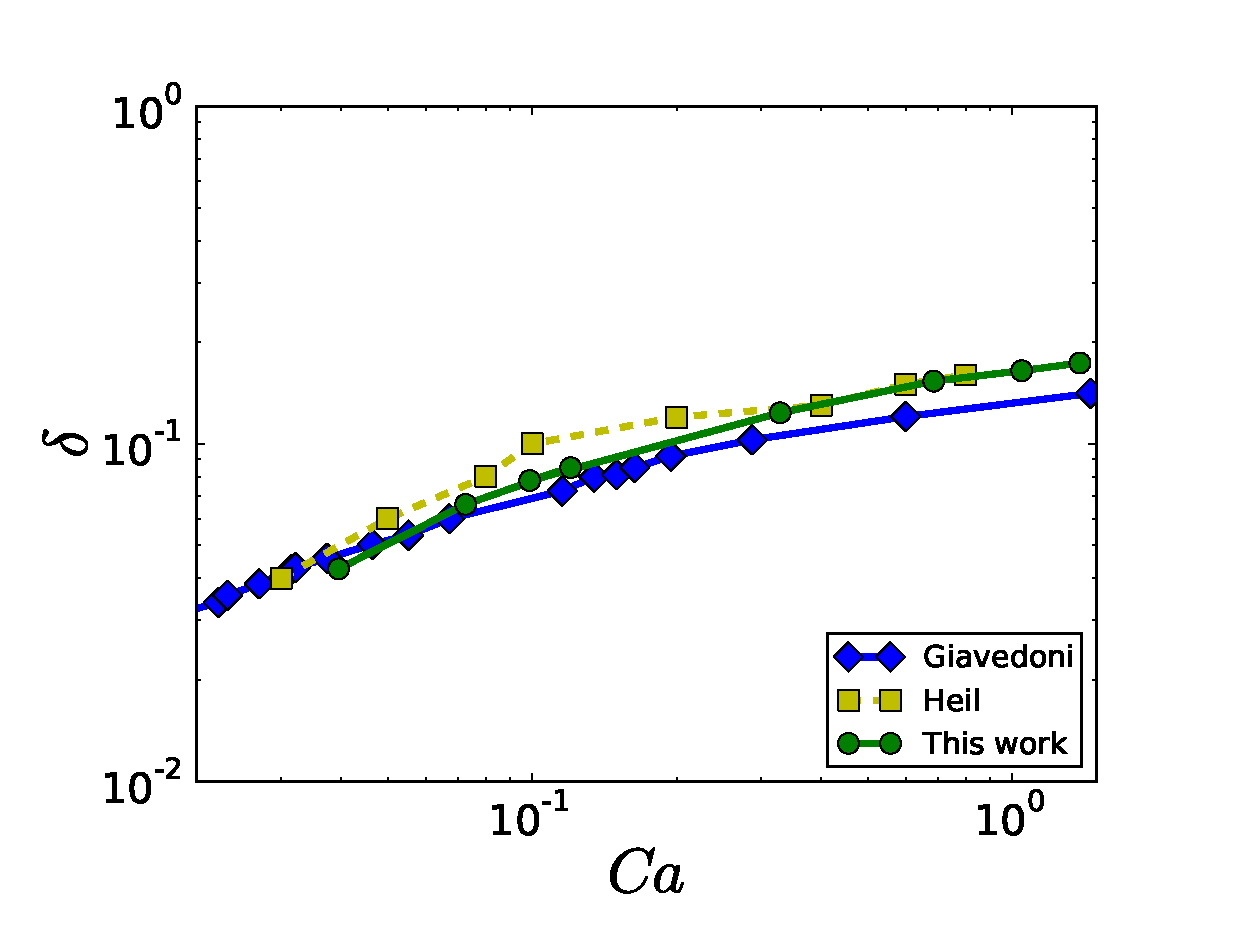
\includegraphics[width=0.5\textwidth]{Figures/capillaries_comparison.eps}
\caption{A comparison between simulation results and results of
\citet{giavedoni-numerical} and \citet{heil-bretherton}. One can see a
reasonable agreement. The plots depict the film thickness as a function of the
the capillary number.\label{fig:capillary:comparison}}
\end{figure}

\begin{table}
\begin{tabularx}{0.5\textwidth}{|X|X|X|X|X|}
\hline
$Ca_{\mathrm{lit}}$&$\delta_{\mathrm{lit}}$&$\delta$&$U_{bubble}$&$Ca$\\
\hline
$0.03$&$0.04$&$0.042$&$0.0022$&$0.039$\\
\hline
$0.05$&$0.06$&$0.066$&$0.0041$&$0.072$\\
\hline
$0.08$&$0.08$&$0.085$&$0.0068$&$0.120$\\
\hline
$0.1$&$0.1$&$0.077$&$0.0055$&$0.098$\\
\hline
$0.2$&$0.12$&$0.123$&$0.0185$&$0.328$\\
\hline
$0.4$&$0.13$&$0.153$&$0.0388$&$0.686$\\
\hline
$0.6$&$0.15$&$0.164$&$0.0592$&$1.046$\\
\hline
$0.8$&$0.16$&$0.173$&$0.0782$&$1.383$\\
\hline
\end{tabularx}
\caption{The parameters and results for capillary number region simulations.
$\delta_{\mathrm{lit}}$ is the film thickness with corresponding $\Ca_{\mathrm{lit}}$ taken from
literature. $\delta_{\mathrm{sim}}$ is the simulation film thickness with corresponding $\Ca$.
$U_{bubble}$ is the bubble interface velocity. $\Ca$ is based on the interface bubble velocity
$U_{bubble}$.
\label{table:parameters:capillary:number}}
\end{table}

\subsection{3D results}
One can see from Fig. \ref{fig:heil:three:dim} that the separation of the axial and diagonal radii
happens at the capillary numbers less than $0.1$. However the axial radius has a value around $0.99
H_{\mathrm{eff}}$. Therefore, the film occupies $0.01 H_{\mathrm{eff}}$ which needs to be resolved
with at minimum $10$ lattice units (see results for grid independency). This condition implies grids
to be of at least size $1000\times1000\times 15000$, which is not a computationally feasible
task. Even the symmetric and antisymmetric profiles are obtained by current simulations, Fig.
\ref{fig:sym:antisym}, the grid independence is not guaranteed.
Therefore our target simulations are from $\Ca\geq 0.1$, where the axial radius equals to the
diagonal radius. In what follows we will show two particular simulations. One is for the dependance
of the bubble radius on the capillary number. Another one is for the velocity patterns. In
comparison with simulations of \citet{heil-threedim} the transition capillary
number is located in the range $0.47<\Ca<0.63$. 
\begin{figure}[ht]
\includegraphics[width=0.5\textwidth]{Figures/sym.eps}\\
\includegraphics[width=0.5\textwidth]{Figures/antisym.eps}\\
\caption{Symmetric ($\Ca=0.63$) and antisymmetric ($\Ca=0.026$) crosssections in the middle of the
bubble. One can see that for the symmetric profile $R_h=R_d$ and for the antisymmetric $R_h\neq
R_d$.  \label{fig:sym:antisym} }
\end{figure}
 
We also simulate only the quarter of the channel by imposing the mirror boundary conditions. This
gives the improvement in memory size and time by factor of four.  
\subsubsection{Capillary region}
We performed a number of simulations with CPU code of grid size $52\times52\times 1500$ for the
quarter of geometry and of refined grid size $82\times82\times 1500$. All other parameters were
chosen as
$k=0.04$,$A=0.04$, and $\Gamma=1.0$. 

The results are presented in Fig.
\ref{fig:capillary:comparison:3d} along with reference data obtained by \citet{heil-threedim}. One
can see that refined grids produce the same results. Thus, the grid of size $52\times52\times 1500$
for the quarter of geometry is enough to obtain grid independent results for $\Ca\geq0.1$. The
capillary number is calculated based on the interface velocity along the center axis. The
simulations results as radii values are underestimated in comparison with the reference data by
\citet{heil-threedim}. This can be explained by the influence of inertia. For example, one can refer
to experimental data obtained by \citet{shikazono-square} with different liquids where real liquid
results can be located below or above the reference curve.
\begin{figure}
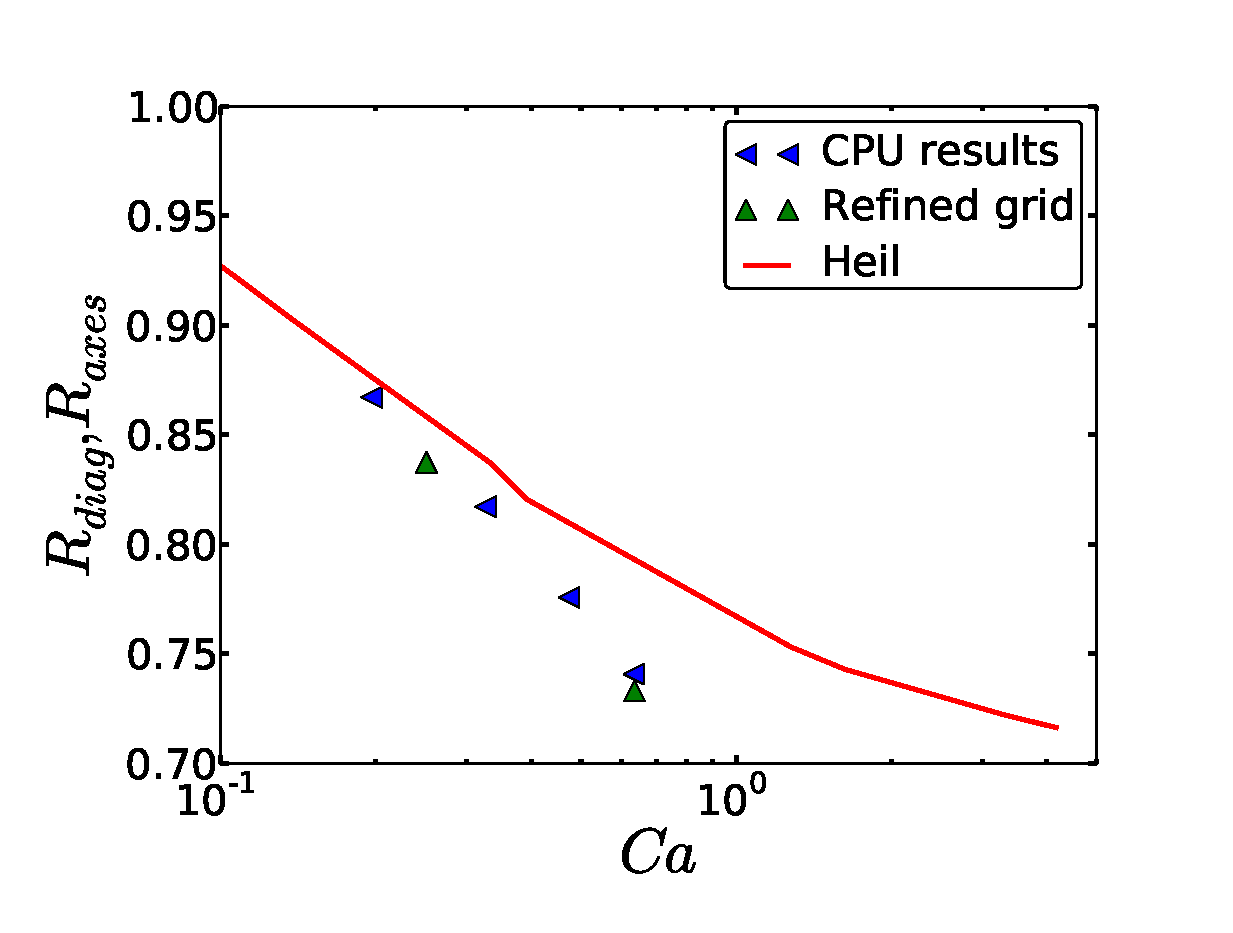
\includegraphics[width=0.5\textwidth]{Figures/capillaries_comparison_3d.eps}
\caption{The comparison between reference data by \citet{heil-threedim} and simulation for the axial
and the diagonal radiuses
versus capillary numbers. One can see that the code mimics
behavior of the earlier published results. The difference can be attributed to the simulation of
binary-liquid instead of the free-surface classical Bretherton
problem. \label{fig:capillary:comparison:3d}}
\end{figure}

\subsubsection{Velocity pattern}
We examined velocity patterns to identify the moment of the streamlines pattern change. We chose two
representative capillary numbers as $Ca=0.47$ and $Ca=0.61$. Scaled velocity profiles in the center
plane are shown  in Fig. \ref{fig:streamlines:pattern}. For demonstration purposes, we restricted
the size of shown velocity vector maps to apply certain scaling and to be able to show the vortex in
the slug. Velocity vector maps are generated in the reference frame of the moving bubble. One can
see a clear transition between associated patterns. The transition capillary number
\cite{heil-threedim} is slightly higher than simulations results. We outline that this fact can be
attributed to the binary-liquid simulations instead of the free-surface classical Bretherton
problem. 
\begin{figure}[!]
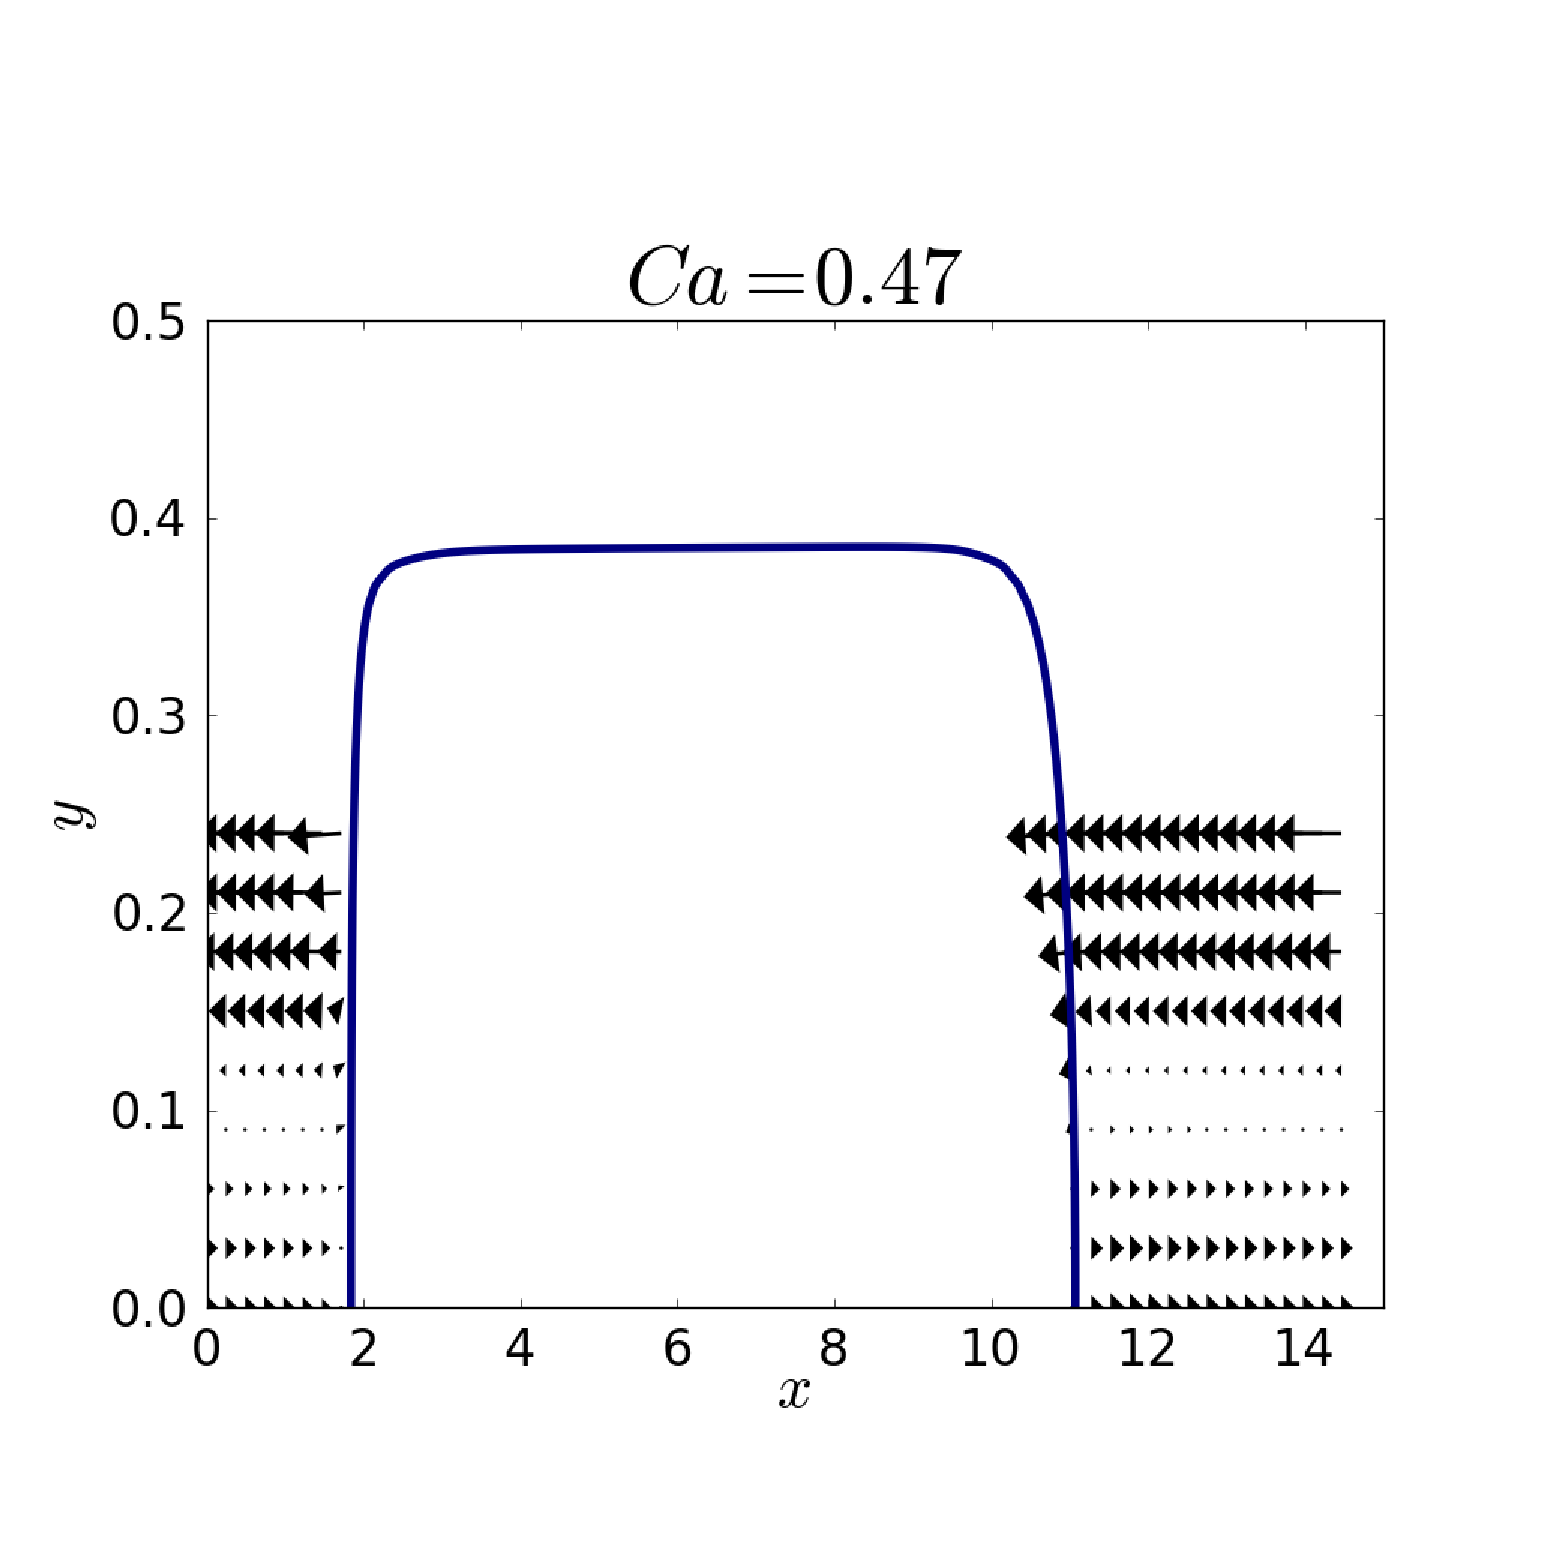
\includegraphics[width=0.5\textwidth]{Figures/vortex_ca47_png.eps}\\
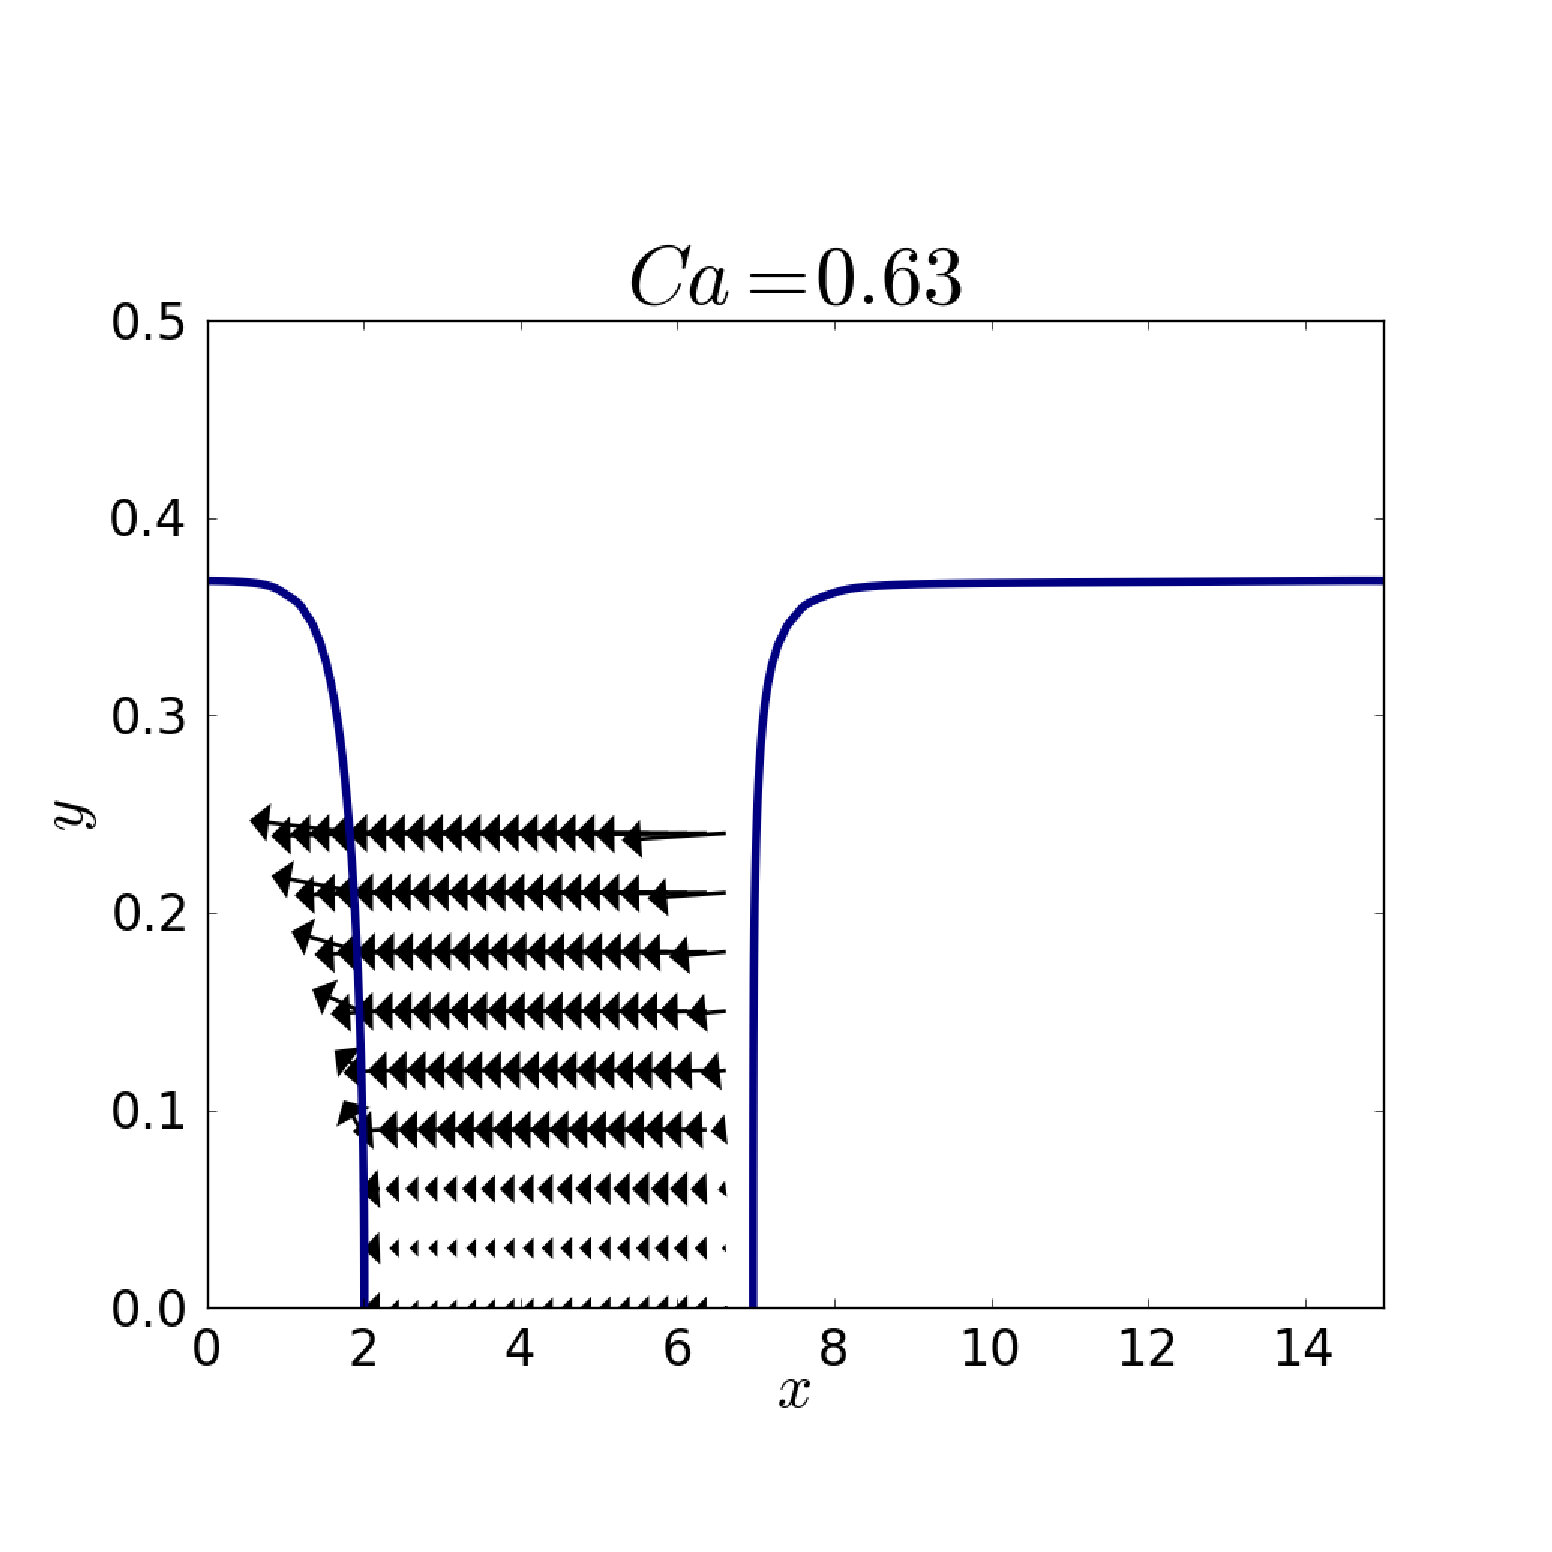
\includegraphics[width=0.5\textwidth]{Figures/vortex_ca63_png.eps}\\
\caption{Velocity vector maps for $\Ca=0.47$ and $\Ca=0.63$. One can see that there are no vortexes
created
before the bubble for $\Ca=0.63$. The transition happens between $\Ca=0.47$ and $\Ca=0.63$, which
is a different value than $\Ca=0.69$ \cite{heil-threedim}. \label{fig:streamlines:pattern}}
\end{figure}

\section{Conclusion}
This work presents numerical studies of the
Bretherton/Taylor problem using the binary liquid lattice Boltzmann method. The bubble was chosen
sufficiently long for the film
thickness to
stabilize, and periodic boundary conditions were used to keep the simulations robust. The
distance between bubbles was taken large enough to minimize
the mutual influence of neighboring bubbles. The computational
results in terms of capillary number dependence and shape of the bubbles show consistency with the
previously published data in two and three dimensions. The simulations show that in the range of low
capillary numbers the
viscous effects dominate over the inertia. The binary liquid model can be used to
simulate gas finger/bubbles propagation in the microchannel. The model is able to catch not only
the film widths but also the velocity patterns change. 
 An examination of the influence of grid resolution on the
results allowed
us to determine that the phase interface should be resolved as at least $50$ percent of the film
thickness
in order for the simulations to be grid independent. Though our results are specific to the binary
liquid lattice
Boltzmann method, the numerical hints and procedures can be used for any
continuous interface method. 

\section{Acknowledgement}
A.~Kuzmin wants to thank Schlumberger for their financial support.
%\newpage

%% %---------------------------
%% %BIBLIOGRAPHY
%% %---------------------------
%The bibliography is created using BiBTeX
\bibliographystyle{CFD2011}
%\bibliography{References}   
\bibliography{paper}
%\newpage
\section{Appendix A}
\label{app:models}
Specific realization of $D2Q9$ and $D3Q15$ models.
\subsection{$D2Q9$ model}
Velocity set is defined as $c_{ix}=\{0,1,0,-1,0,1,-1,-1,1\}$ and $c_{iy}=\{0,0,1,0,-1,1,1,-1,-1\}$.
Parameters specific to the D2Q9 grid are the weights
$w_i=\left\{\frac{4}{9},\frac{1}{9},\frac{1}{9},\frac{1}{9},\frac{1}{9},
\frac{1}{36},\frac{1}{36},\frac{1}{36},\frac{1}{36}\right\}$.  The weights related to the
inclusion of the surface tension coefficient into the equations are as follows:
$w^{xx}_{1-2}=w^{yy}_{3-4}=1/3$, $w^{xx}_{3-4}=w^{yy}_{1-2}=-1/6$,
$w^{xx}_{5-8}=w^{yy}_{5-8}=-1/24$, $w^{xy}_{1-4}=0$, $w^{xy}_{5-6}=1/4$ and
$w^{xy}_{7-8}=-1/4$.

\subsection{$D3Q15$ model}
Velocity set is defined as:
\begin{equation} 
\begin{aligned}
&c_{ix}=\{0,1,-1,0, 0,0, 0,1,-1, 1,-1,0, 0, 0, 0,1,-1, 1,-1\}\\
&c_{iy}=\{0,0, 0,1,-1,0, 0,1, 1,-1,-1,1,-1, 1,-1,0, 0, 0, 0\}\\
&c_{iz}=\{0,0, 0,0, 0,1,-1,0, 0, 0, 0,1, 1,-1,-1,1, 1,-1,-1\}.
\end{aligned}
\end{equation}
The weights are $w_0=0$, $w_{1-6}=\frac{1}{6}$ and $w_{7-18}=\frac{1}{12}$. The weights
related to the inclusion of the surface tension are:
\begin{equation}
\begin{aligned}
&w^{xx}_{1-2}=w^{yy}_{3-4}=w^{zz}_{5-6}=\frac{5}{12}\\
&w^{xx}_{3-6}=w^{yy}_{1-2,5-6}=w^{zz}_{1-4}=-\frac{1}{3}\\
&w^{xx}_{7-10,15-18}=w^{yy}_{7-14}=w^{zz}_{11-18}=-\frac{1}{24}\\
&w^{xx}_{11-15,}=w^{yy}_{15-18}=w^{zz}_{7-10}=\frac{1}{12}\\
&w^{xy}_{7,10}=-w^{xy}_{8,9}=w^{yz}_{11,14}=-w^{yz}_{12,13}=w^{zx}_{15,18}=-w^{zx}_{16,17}=\frac{1}{
4}.
\end{aligned}
\end{equation}


\end{document}